% Setup - do not change
\documentclass[11pt]{article}
\usepackage[top=0.9in, left=0.9in, bottom=0.9in, right=0.9in]{geometry} 
\usepackage{parskip}

\usepackage[english]{babel}
\usepackage[utf8]{inputenc}
\usepackage{amsmath,amsthm,amssymb,graphicx,pdfpages,lipsum,hyperref}
\usepackage[none]{hyphenat}
\usepackage{csquotes}
\usepackage{paralist}
\usepackage{enumitem}
\usepackage{graphicx}
\usepackage{subfigure}
\usepackage{booktabs}
\usepackage{amsmath}


\setlength\parindent{0pt}
%%%%%%%%%%%%%%%%%%%%%%%%%%%%%%%%%%%%%%%%%%%%%%%%%%%%%%%%%%%%%%%%%%%
% add other packages here if required

%% Bibliography are specified in this file. You can also choose inline bib style if you want to. But make sure your citation style is consistent (and proper)
% For more details on citation: https://library.unimelb.edu.au/recite
\usepackage[sorting = none]{biblatex}
\addbibresource{references.bib}

%%%%%%%%%%%%%%%%%%%%%%%%%%%%%%%%%%%%%%%%%%%%%%%%%%%%%%%%%%%%%%%%%%% the '%' symbol denotes comments

% Begin document creation
% DELETE THE \lipsum PLACEHOLDERS WHEN YOU BEGIN
\title{Comprehensive analysis on tip amount of Yellow Taxi in NYC}
\author{
Cheng Qian \\
Student ID: 1266297 \\
%% Replace the link with your github repo
% 1. Remember to escape underscore (\_) in the link.
% 2. Remember to include the commit you want to submit in the link
\href{https://github.com/ChrisQian6/MAST30034_Python}{Github repo with commit}
}

\begin{document}
\maketitle

\section{Introduction}
% Link to a 30 min tutorial if you require revision: https://www.overleaf.com/learn/latex/Learn_LaTeX_in_30_minutes

The trend of online taxis gradually replacing traditional taxis has become more and more apparent over the past few years. As shown in Figure 1, in January 2023, only three million trips were recorded for taxis in New York City, U.S.A., whereas there are nearly 20 million for online taxis. It is because it explores the impact of mobile internet and smartphones driving the rise of ride-hailing services, enhancing the experience of booking rides. Secondly, it discusses the flexibility and convenience offered by ride-hailing platforms, challenging the traditional taxi model. Moreover, it addresses the labor rights concerns for ride-hailing drivers, emphasizing the importance of balancing economic benefits and labor rights. In conclusion, the rise of ride-hailing services is influenced by factors such as technology, convenience, and labor rights, and relevant regulations should adapt to the evolving landscape.


\begin{table}[ht]
\centering
\begin{tabular}{|c|c|c|c|}
\hline
No. YellowTaxi & No. GreenTaxi & No. ForHireVehicle  & No. HVForHireVehicle\\
\hline
3066766 & 68211 & 1114320 & 18479031 \\
\hline
\end{tabular}
\caption{Number of trips recorded by different taxi firms}
\end{table}


Taken together, taxi companies and drivers face challenges and opportunities under the trend of online taxi substitution. Taxi companies must adapt to the new market environment and adopt innovative business strategies to maintain competitiveness. Drivers, on the other hand, need to weigh factors such as job flexibility, income stability, as well as regulatory and insurance issues, to make decisions that suit their circumstances.\cite{industry}

In this paper, I examine in detail the trip logs of New York City taxis and do an \textbf{in-depth study of the tips that taxi riders pay to their drivers for the reference of taxi drivers as well as taxi companies}. Due to concerns about being affected by the COVID period, I picked \textbf{the most recent update of six months of data}, as well as being able to ensure that my research was up to date.  Due to different service areas and focus, the records for green taxis are almost 90 percent less than those for yellow taxis shown in Table 1. (Green taxis primarily operate outside of the Manhattan area, serving places like the Bronx and Queens. The demand in these areas might be lower than in Manhattan, leading to fewer green taxis). Therefore, only the records of yellow taxis are selected to do research.\cite{tlc}

\section{Preprocessing}
This process refers to the series of steps taken to clean, transform, and organize raw data into a format suitable for analysis and modeling. It's a crucial initial phase that enhances the quality and reliability of the data, making it ready for further exploration and modeling. Preprocessing ensures that the data is consistent, accurate, and suitable for effective analysis and machine learning.

\subsection{Adding New Features}
As the current 19 features may not be very relevant for analyzing and predicting the tip amount or are stored in an inadequate form, we need to generate the features we need by extracting or transforming these pre-existing features. The following attributes are added:

\begin{itemize} 
    \item \textbf{‘Datetime'}. This is extracted from the existing ‘pick up time’ column, which indicates the year, month, and date of the trip. This is used to merge the external dataset which would be introduced later in the report.
    \item \textbf{‘Duration’}. This is calculated by subtracting pick-up time from drop-off time, indicating the duration of the trip in seconds.
    \item \textbf{‘hourly\textunderscore earn’}. This is calculated by the total amount paid by the passenger divided by the duration of the trip in hours, indicating the revenue efficiency of the trip.
    \item \textbf{‘Month’ and ‘Hour’}. This is extracted from the existing ‘pick up time’ column, which indicates the month of the trip and the hour of the day.
    \item \textbf{‘Weekend’}. This is extracted from the existing ‘pick up time’ column, which is a boolean datatype that indicates the trip took place whether on the weekend or not.
    \item \textbf{‘Airport’}. This is extracted from the existing ‘airport fee’ column, which is a boolean datatype that indicates the trip whether passed through the airport or not. This is because 1.25 dollars is charged if you pass through the airport, not if you don't. So the feature ‘airport fee’ itself is a boolean format data, there is no need to store it in double format.
    \item \textbf{‘Congestion’}.  This is extracted from the existing ‘congestion fee’ column. Dealing with this feature in the form of a double may not be very relevant for what we are analyzing, but in the form of a boolean may alleviate the model complexity to achieve the desired result.
\end{itemize} 

\subsection{Feature Selection}
Feature selection refers to the process of selecting the most relevant and useful features from the original feature set of data for analysis, modeling, and prediction tasks. Feature selection is an important step in data preprocessing that helps improve model performance, reduce overfitting risks, and lower computational costs. The raw data included 19,585,935 pieces of the instance. The following steps were taken to filter non-relevant or unusual instances:
\begin{itemize} 
    \item \textbf{Uncommon trip durations and distances} are removed. These include trips of less than one minute or more than five hours, and trip distances that are negative or exceed 280 miles (the maximum distance a normal car can travel on a full tank of fuel). These data are very uncommon, even strange. If retained they may be used as outliers to influence the analysis that follows.
    \item \textbf{Negative amount for fare amount, tips, and other fees-related columns} are removed. Similar to the above, the topic of this report is also related to fees. It is therefore extremely crucial to remove the outliers on fees-related features.
    \item \textbf{Passenger counts that are negative} are removed. Contrary to the thinking of many, data with zero passengers will be retained. This is because many people today take taxis many times just to deliver an item to another person and do not carry any passengers. And let's assume that people who take a taxi to deliver an item often need the cooperation of the driver to get it to the recipient. So the tip received may tend to be higher.
    \item \textbf{Payment methods other than credit card} are removed. As mentioned in the data dictionary, this field is automatically populated for credit card tips. Cash tips are not included. 
    \item \textbf{Instances with null value} in it are removed. After doing a preliminary look at the data, we found that instances that do not contain null values make up 97\% of all data. Therefore, it was concluded that removing 3\% of the data containing null values would not have a significant impact on the overall distribution.
\end{itemize} 

After a round of screening, 22.8\% of instances in the original raw data are removed, leaving 15,121,628 valid data eventually left to do in-depth research.

\subsection{Merging External Dataset}
In addition, we believe that the weather conditions at the time of the taxi ride may have some degree of influence on the tip paid by the passenger. Therefore data on temperature, rainfall, and other such weather types (from \href{https://www.visualcrossing.com/}{VisualCrossing}) were imported into the current dataset to aid in the study of our topic with the following attribute \cite{weather}(in days):


\begin{center}
\begin{tabular}{@{}llll@{}}
$\bullet$ Average Temperature \qquad & $\bullet$  precipitation \qquad  & $\bullet$ Wind speed \qquad & $\bullet$ Visibility\\
\end{tabular}
\end{center}



\section{Preliminary Analysis and Geospatial Visualization}
This section refers to a series of foundational steps and exploratory analyses conducted before delving into in-depth data analysis. These steps help in understanding the basic characteristics, trends, and outliers, which prepares the ground for more advanced analyses and modeling. (Null values are removed as mentioned above)

\subsection{Distribution}
When conducting data analysis, plotting the distribution of the label under investigation is helpful in gaining insights into the data's characteristics, thereby providing crucial guidance for subsequent analysis and modeling. As shown in Figure 1(a), which is the distribution of tip amount in the sample dataset, there are a few outliers when tip amounts are large. This results in a strongly right-skewed distribution. After removing these outliers in Figure 1(b), we can observe that the overall skewness is mitigated. After careful deliberation from the distribution of the sample data, it was decided that instances with tip amount greater than \$120 are removed as outliers. 

\begin{figure}[t]
    \centering
    \subfigure[All sample data]{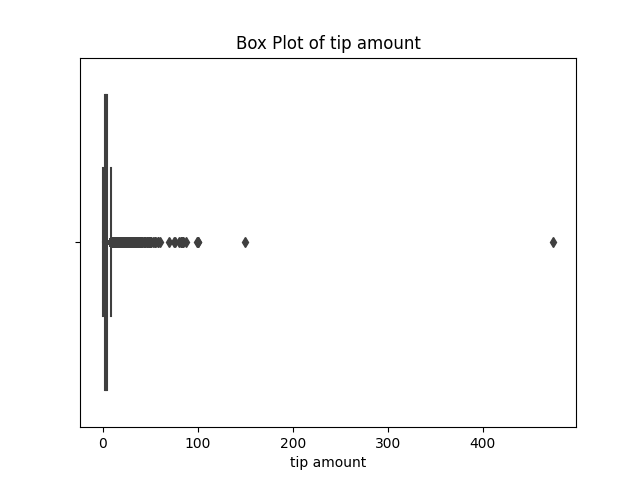
\includegraphics[width=0.45\textwidth]{box_plot_tipamount.png}} 
    \subfigure[Outliers removed data]{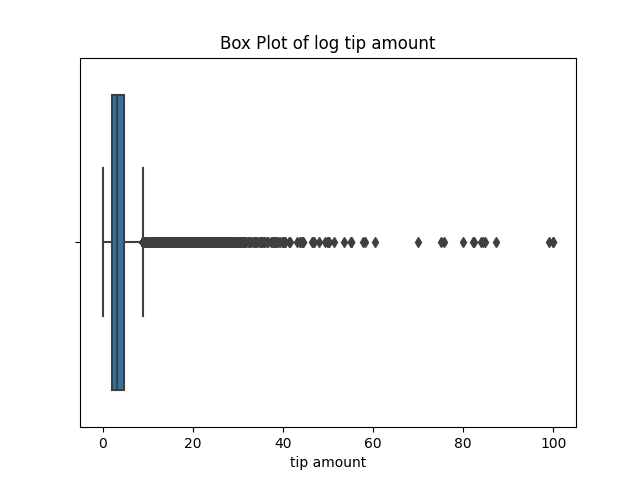
\includegraphics[width=0.45\textwidth]{box_plot_tipamount_removedoutlier.png}}
    \caption{Box plot of tip amount}
    \label{fig:foobar}
\end{figure}

We are moving on to the distribution of a more general amount of tips, which is between \$0 to \$17. Finding out the distribution of them results in clearer and more meaningful interpretations of the relationships among the variables, allowing for better insights, which also derive better generalization. 

\begin{figure}[t]
    \centering
    \subfigure[Original distribution]{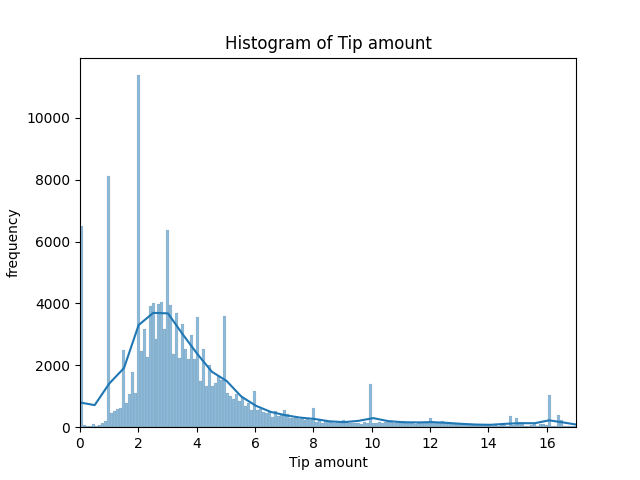
\includegraphics[width=0.45\textwidth]{tip_histogram.png}} 
    \subfigure[Log transformed distribution]{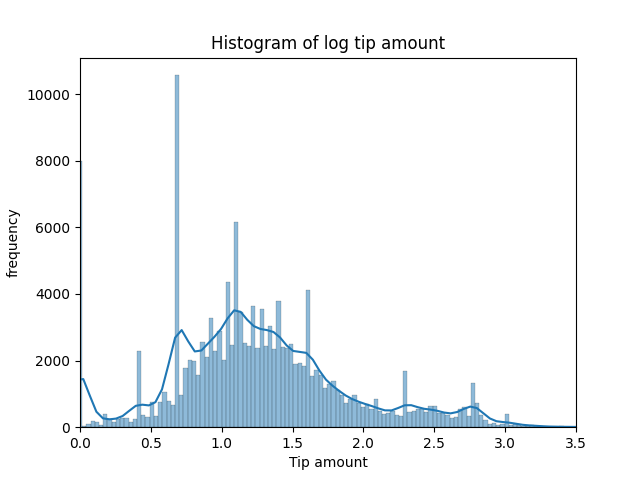
\includegraphics[width=0.45\textwidth]{log_tip_histogram.png}}
    \caption{Histogram of tip amount}
    \label{fig:foobar}
\end{figure}

From Figure 2(a) we can observe that the image remains skewed to the right, even for the more general range of tip amount. It can also be observed that tip amounts that are integers all bulge out from the image, especially when they are \$1 and \$2. After some investigation, this is because, on the payment terminal, there will likely be a prompt asking if you'd like to add a tip for the driver. You can choose the tip amount, often provided as an integer, and a small amount such as \$1 or \$2 would usually be tipped by the passenger. Unlike when paying in cash, people would tip the driver with the change in their pockets, so it will rarely be an integer. 

Since the analysis and modeling following require the assumption that the data is normally distributed. However, the distribution of the tip amount is right skewed. Therefore we need to log the transformation to the tip amount. In Figure 2(b), we notice that the transformed data mainly conforms to a normal distribution, although there are still many bumps.

\subsection{Correlation Between Features}

In data analysis, a  heat map is a visualization tool that represents a data matrix using colors, making complex data patterns, relationships, and trends more intuitive and understandable.  Each cell's color represents the magnitude of the corresponding data value or feature. This visualization method helps uncover patterns, similarities, and differences among data, providing valuable information for decision-making.

\begin{figure}[h]
    % change the scale multiplier to make the figures smaller or larger
    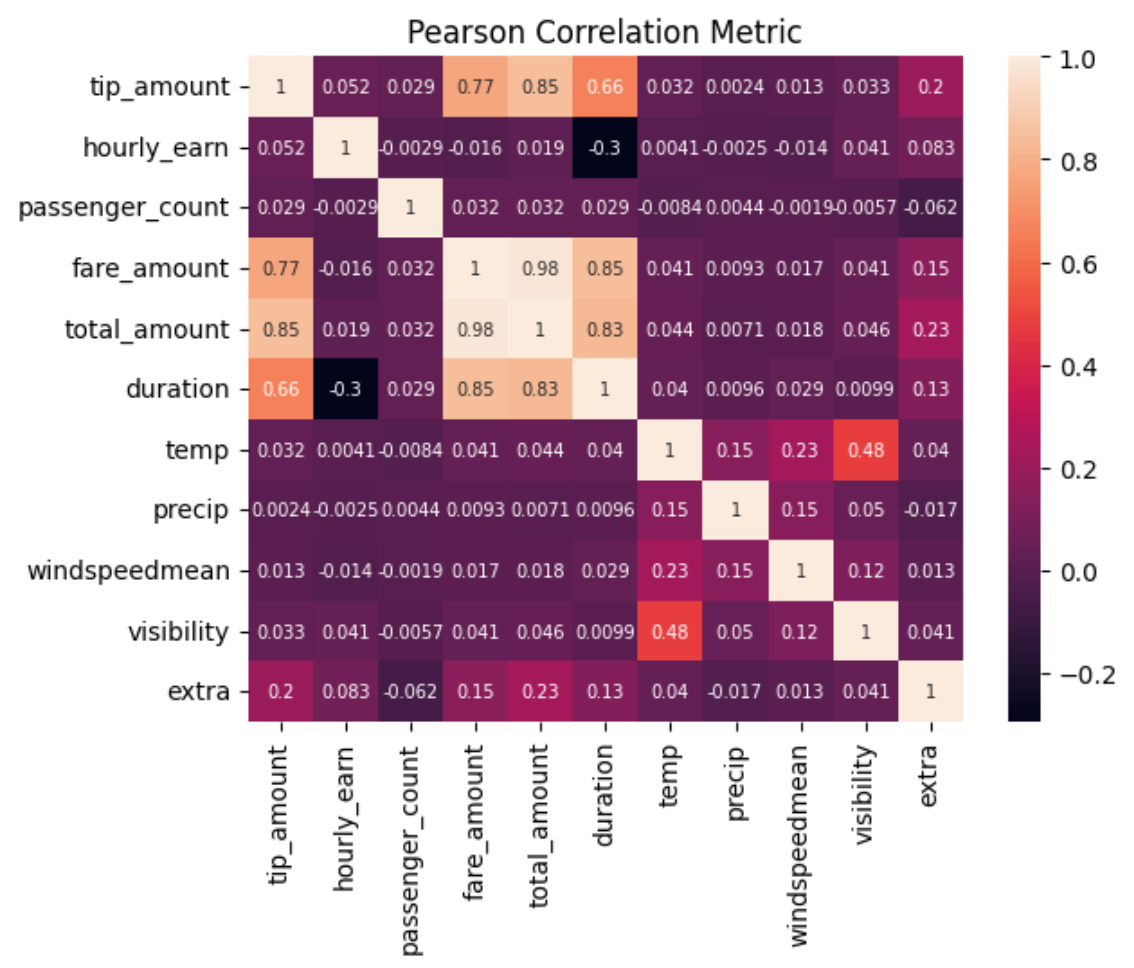
\includegraphics[width=0.8\textwidth]{heatmap.png}
    % this ensures your figures are centered where possible
    \centering
    \caption{Heat map of features} % refer to this image as (Figure 1)
\end{figure}

The heat map in Figure 3 shows the correlation between all the numerical data in the dataset.
Unlike the assumptions made in the preprocessing phase, we can observe that weather data such as temperature, precipitation, wind speed, and visibility have no effect on the number of tips paid by passengers. This is a significant impact on this study, as the previously imported external dataset is likely to perform poorly for this study. 

In the available dataset, we can recognize the high correlation between the tip amount and the fare amount, the total amount, and the duration from the heat map. If there is a high correlation among exploratory variables, it might lead to multicollinearity issues. Multicollinearity can affect the stability and interpretability of the model. In this case, examining the correlations between exploration variables is significant. The reason fare amount and tip amount are highly correlated with the total amount is that they are both included in the total amount with other fees such as airport or congestion fees. And it is common sense that when the duration of the ride is longer, the cost will be higher, which explains the correlation between those fees-related columns. Hence, we only need duration to explore the relationship with tip amount.

\begin{table}[ht]
\centering
\begin{tabular}{@{}lccccc@{}}
\toprule
Source of Variation & Sum of Squares & Degrees of Freedom & F-Value & p-value \\
\midrule
Weekend & 74.797129 & 1.0 & 236.656787 & 2.323348e-53 \\
Airport & 74.239905 & 1.0 & 234.893739 & 5.622621e-53\\
Congestion & 1663.384381 & 1.0 & 5262.918614 & 0\\
PULocationID & 2147.208404 & 154.0 & 44.115125 & 0\\
DOLocationID & 9174.217908 & 242.0 & 119.946539 & 0\\
Total & 45640.585104 & 144406.0 & & \\
\bottomrule
\end{tabular}
\caption{ANOVA Table}
\end{table}

For those categorical features such as whether the trip passes through an airport, whether it's on a weekend, and whether it's congested, the ANOVA shown in Table 2 demonstrates that relationship. We discover that the probability that these features have no relevance to tip amount is extremely small. It can also be concluded that the pickup and drop-off location of a trip has a strong correlation with the tip amount received. 

\subsection{Geospatial Analysis}

\begin{figure}[t]
    \centering
    \subfigure[pick-up]{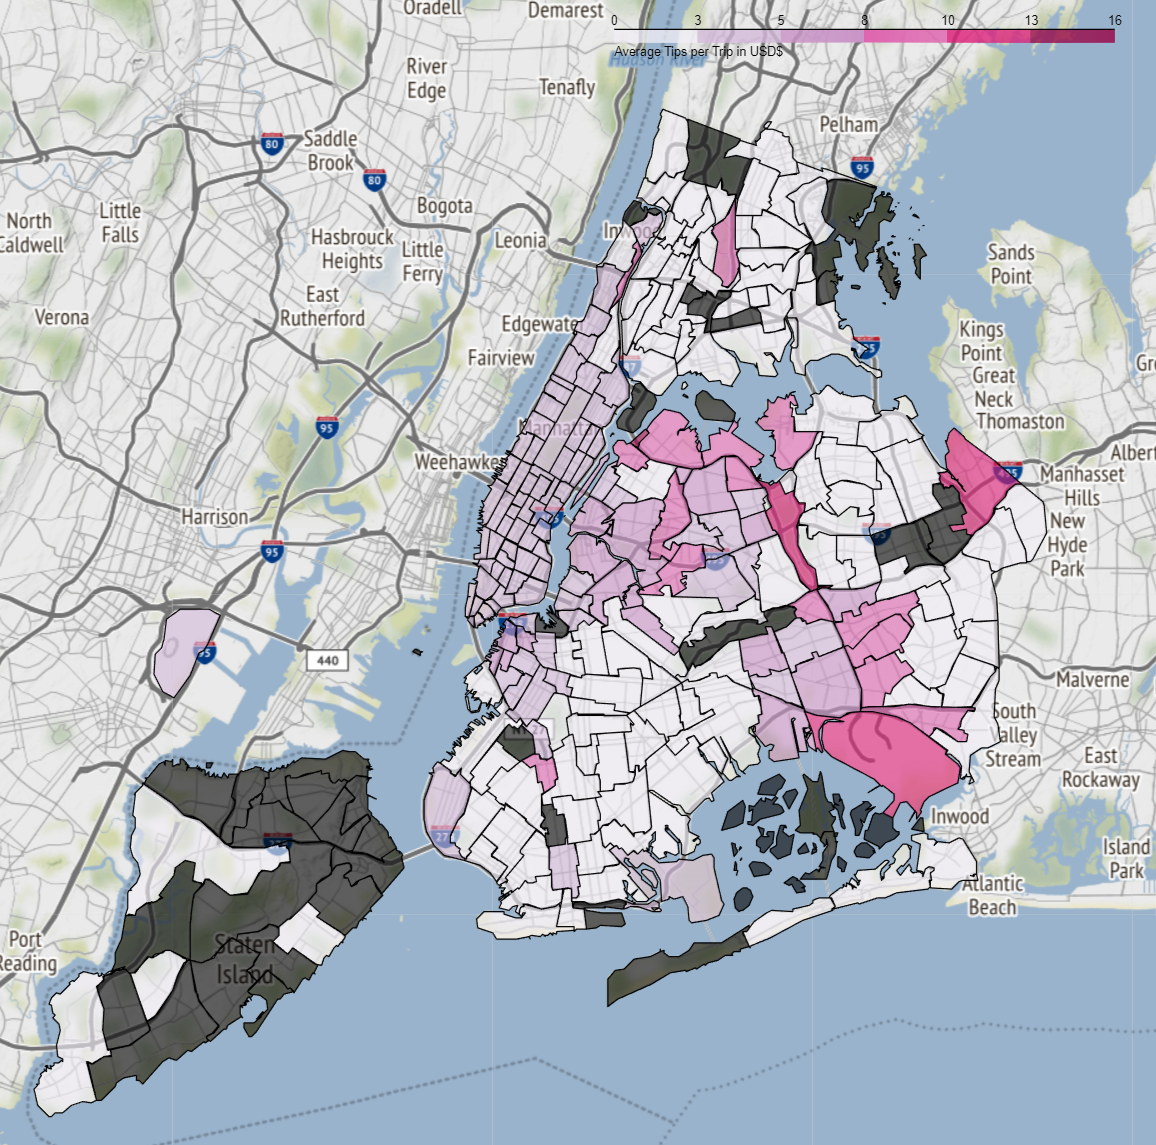
\includegraphics[width=0.49\textwidth]{pickup_tip.png}} 
    \subfigure[drop-off]{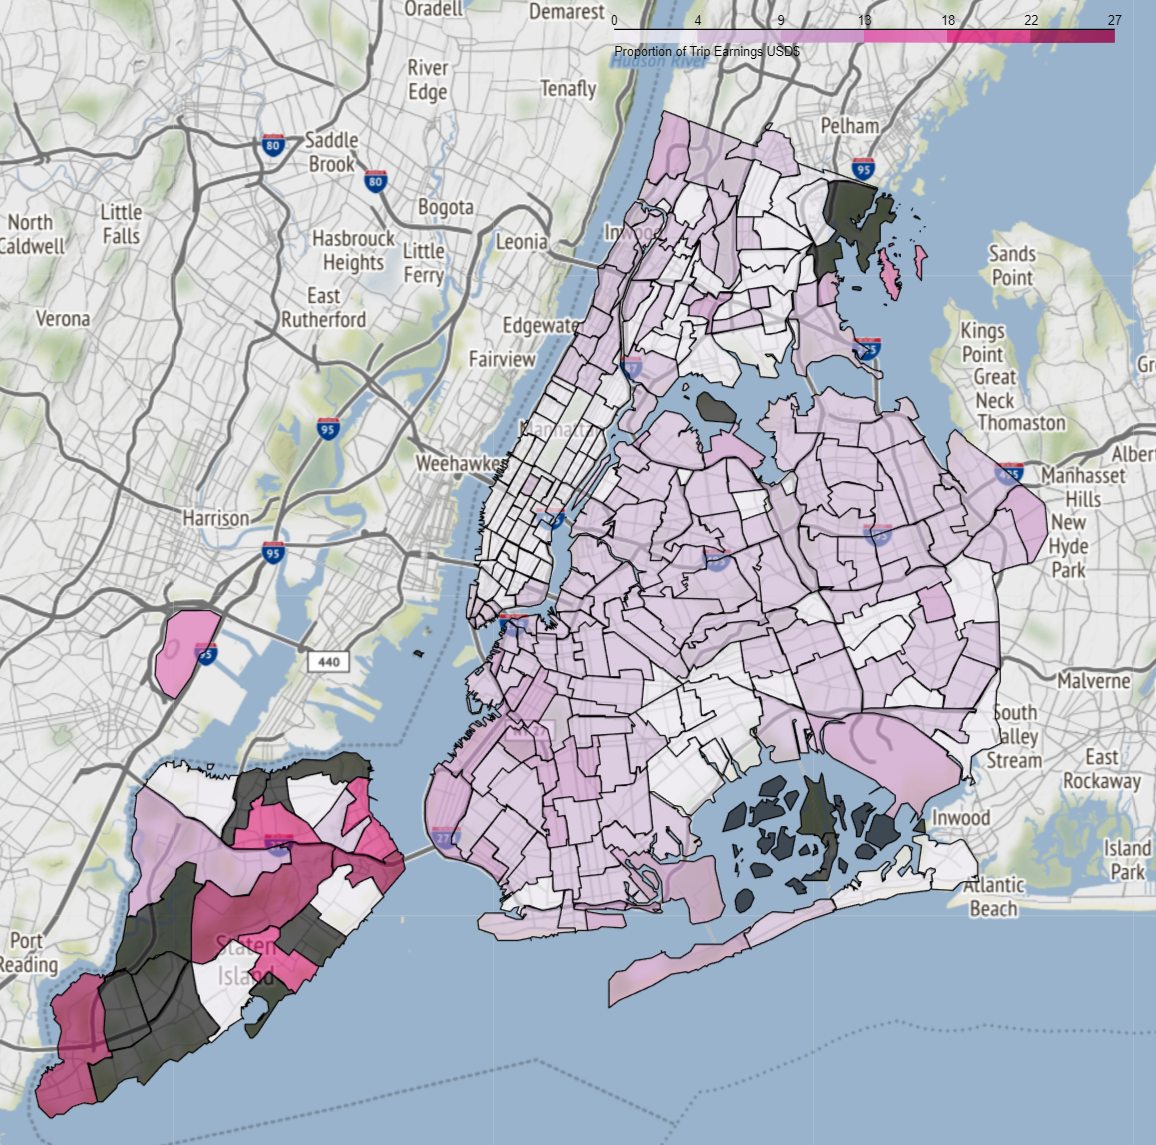
\includegraphics[width=0.49\textwidth]{dropoff_tip.png}}
    \caption{Average tips per trip in different locations}
    \label{fig:foobar}
\end{figure}

Figure 4 demonstrates the average tip amount per trip for different locations. It can be observed that the average amount of tips paid by passengers is relatively high if the pick-up point is in Flushing Meadows Corona Park and Flushing (NY 11362), or if the drop-off point is in most areas of Staten Island, as well as if picking up or dropping off on the airport (John F. Kennedy International Airport (JFK), LaGuardia Airport (LGA), and Newark Liberty International Airport (EWR) ), which verifies whether passing through the airport is related to tip amount.

\section{Modeling}
The modeling step serves a crucial purpose. Its primary objective is to construct a mathematical model to extract relationships and trends from the data. This allows us to make predictions for tip amounts, and aid in decision-making. Selecting the appropriate models  would transform data into useful information and insights and optimize resource allocation. 

The data is split 80\% into training data and 20\% into testing data, which helps accurately evaluate model performance, preventing overfitting and enhancing the ability of generalization.

\subsection{Linear Regression Model}
Linear regression is a commonly used regression analysis method in the fields of statistics and machine learning. It is employed to establish and predict a linear relationship between one or more independent variables and a dependent variable. It assumes a linear relationship between the independent and dependent variables, meaning that the changes in the dependent variable can be explained by a linear combination of the independent variables.\cite{lr}

Among the available features, after examining their correlation to tip amount, two features, duration and extra, were chosen as numeric data, and three features, passing through the airport or not, congested or not, and whether it was a weekend or not, were chosen as categorical data to predict the number of tips.

\subsection{Random Forest Classifier Model}
The random forest classifier model is used for classification tasks and it is a versatile and powerful model widely used in various domains due to its ability to handle complex datasets, prevent overfitting, and deliver accurate predictions.\cite{rf}

In this case, the tip amount is divided into two categories, low tips and high tips (less than or equal to \$3 is a low tip, otherwise a high tip). In the selected features, in addition to the three categories of airport, weekend, and congestion features used in the linear regression, two categories of pick-up and drop-off locations were added, for a total of five categorical features for the training data.

\subsection{Results and Error Analysis}
RMSE (Root Mean Squared Error), which is an indicator to evaluate the performance of linear regression, is adopted in this study. It measures the error between the model's predicted value and the actual observed value. After hyperparameter tuning and selecting the best-performing model, the \textbf{RMSE value is approximately 2.7983}, and \textbf{the R squared value $\approx$ 0.4741}. (An R-squared value of 0.4741 indicates that approximately 47.41\% of the variability in the dependent variable is explained by the linear regression model.) The overall modeling performance generally meets expectations.

\begin{table}[ht]
\centering
\[
\begin{array}{c|cc}
& \text{Predicted High Tips} & \text{Predicted Low Tips} \\
\hline
\text{Actual High Tips} & 205941 & 1116143 \\
\text{Actual Low Tips} & 113656 & 1590587 \\
\end{array}
\]
\caption{Confusion Matrix}
\end{table}

\begin{center}
    
Recall = $\frac{TP}{TP + FN}$ , \quad Precision = $\frac{TP}{TP + FP}$

\small{Note: TP = Correctly predicted high tip, FN = Predicted low tip but Actually high tip, \\
TN = Correctly predicted low tip, FP = Predicted high tip but Actually low tip.}
\end{center}
As random forest is a classification model, we would employ different evaluation methods. As shown above, the confusion matrix is a tabular representation to evaluate the performance of a classification model. it provides a clear visualization of how well our model's predictions align with the actual ground truth. After calculation, we derive that the Precision $\approx$ 0.13 and Recall $\approx$ 0.63 (The formula is shown above). The low precision, in this case, indicates that when the model predicts a high tip, it is likely to be incorrect. However, the high recall indicates that the model is effective at identifying high-tip instances, but it may lead to more false positives. Regardless, this model ends up being equal to about 60\% Accuracy, so it's still relatively reliable.

\section{Recommendation}
In this study, we can directly summarize from it that the following conditions are all effective in increasing trip tipping:
\begin{itemize}


    \item \textbf{Passing through airports}
    \item \textbf{On a weekend}
    \item \textbf{Through congested roads}
    \item \textbf{Picking up or dropping off at a specific location shown in Figure 4}
    \item \textbf{The longer the trip, the higher the tip}
\end{itemize} 
In addition, based on the two mathematical models presented in the overview, we can compare the degree of confidence in the reliability of their predictions of the tip amount. We recommend that your company enhance the training of the model with internal datasets and refine it to be added as a piece of software or an app to the cab itself or to the cab driver's cell phone. This will increase the income of the drivers, thus attracting more drivers to stay in the taxi industry and mitigating the accelerating trend of online taxis taking over the cab industry in recent. 

\clearpage

\printbibliography

\end{document}
 